%Como se juntan las definiciones con lo demás
\section{Metaheurísticas aplicadas al JSP}
La complejidad del JSP hace que las metaheurísticas sean actualmente los métodos más utilizados para resolver instancias grandes. 
%
Estas han conseguido hallar buenas soluciones para los conjuntos de prueba más populares. 
%
Se han empleado una gran variedad de metaheurísticas como: algoritmos genéticos~\cite{Cheng1999}, evolución diferencial~\cite{Ponsich2013}, 
algoritmos de colonia de hormigas~\cite{Klc2007}, algoritmos de enjambre de partículas~\cite{zhang2019novel} y búsqueda tabú~\cite{Zhang2007}. 
%
Aunque estos son algoritmos muy diferentes entre sí, la mayoría de ellos o extensiones de los mismos, aplican de alguna forma el concepto de 
búsqueda local para mejorar su desempeño.
%
Otro punto en común es que la mayor parte de algoritmos trabajan con la representación basada en permutaciones con soluciones semi-activas, y que se cuentan con múltiples vecindades para este tipo de representación.

Para aplicar el proceso de búsqueda local es necesario introducir una definición de vecindad, como se ha mencionado anteriormente esta estructura es parte 
del paisaje de búsqueda y tiene un gran impacto en los resultados obtenidos. 
%
A lo largo del tiempo se han propuesto diversas vecindades cada vez con mejores resultados. 
%
A continuación se presentan las vecindades más importantes hasta la fecha. 


\subsection*{Vecindades previamente propuestas}
Todas las vecindades presentadas aquí se basan en el concepto de ruta crítica y solo consideran cambios dentro de los bloques críticos. Esto implica que estas vecindades están pensadas exclusivamente para soluciones semi-activas.
%
En las figuras siguientes se presentan figuras ilustrativas para cada una de estas definiciones.

\begin{itemize}
\item N1~\cite{blazewicz1996job}: Consiste en considerar todas las soluciones que se crean al intercambiar cualquier par de operaciones adyacentes que pertenecen 
a un bloque crítico. Aunque esta vecindad no es particularmente grande ya que es aproximadamente del tamaño de la ruta crítica, considera muchos cambios para los que 
actualmente se tienen demostraciones de que no pueden mejoran el makespan, por lo que en la actualidad prácticamente no se utiliza.
\begin{figure}[H]
\centering
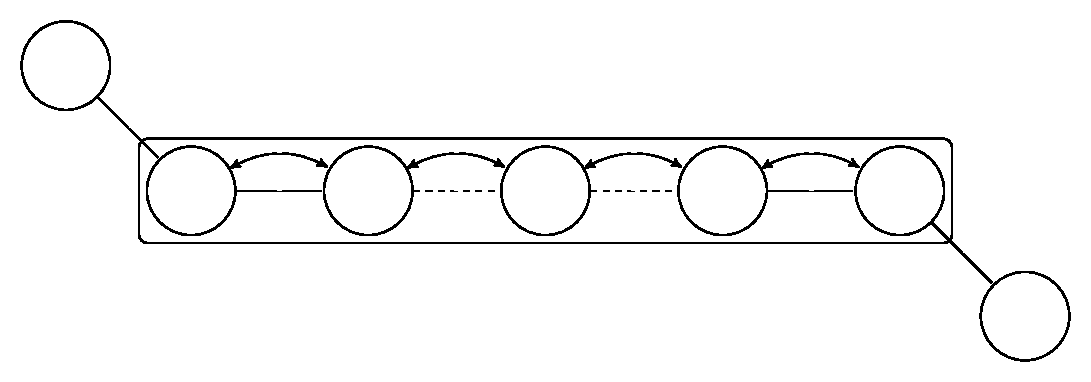
\includegraphics[scale=.7]{Imagenes/N1.pdf}
\caption{Movimientos de la vecindad N1}
\end{figure}

\item N4~\cite{dell1993applying}: Esta vecindad se propuso como un refinamiento y extensión de la vecindad N1 y toma como base el concepto de bloque crítico. 
%
Consiste en llevar operaciones internas del bloque crítico al inicio o final. 
%
Esta vecindad es de tamaño comparable a la anterior pero presenta movimientos más perturbativos.
\begin{figure}[H]
\centering
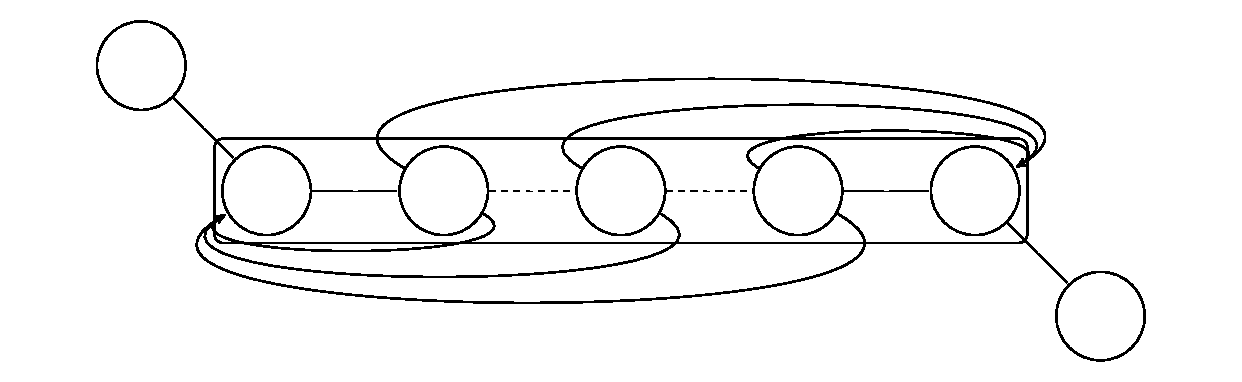
\includegraphics[scale=.7]{Imagenes/N4.pdf}
\caption{Movimientos de la vecindad N4}
\end{figure}


\item N5~\cite{EugeniuszNowicki2003}: Consiste en intercambiar solo las operaciones adyacentes a la final o inicial de un bloque crítico. 
%
Es aun más pequeña que la anterior ya que es aproximadamente del tamaño del número de bloques críticos, así que se puede utilizar para casos muy grandes, y si se desea
reducir el costo computacional.
\begin{figure}[H]
\centering
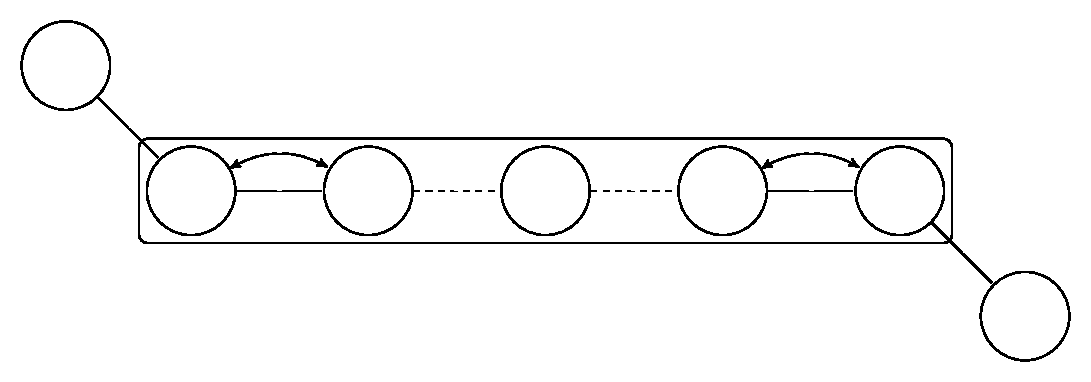
\includegraphics[scale=.7]{Imagenes/N5.pdf}
\caption{Movimientos de la vecindad N5}
\end{figure}

\item N6~\cite{Balas1998}: Los autores utilizan varios teoremas para identificar pares $(u,v)$ de operaciones dentro de un bloque crítico que puedan llevar a mejorar la 
solución y a su vez identificar si se tiene que mover a $u$ justo después de $v$(forward) o bien a $v$ justo antes de $u$ (backward). 
%
Esta vecindad puede verse como un refinamiento y extensión de la N4 por lo que tiene un tamaño similar.
\begin{figure}[H]
\centering
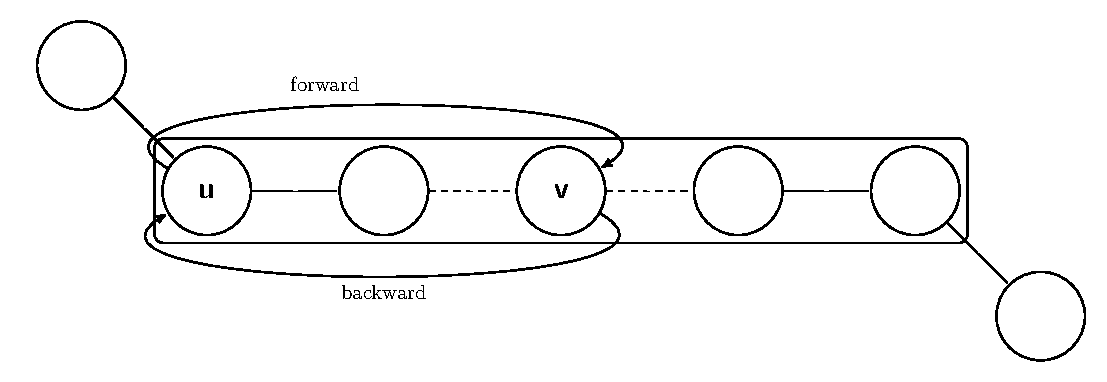
\includegraphics[scale=.7]{Imagenes/N6.pdf}
\caption{Los dos tipos de movimientos para un par $(u,v)$}
\end{figure}

\item N7 \cite{Zhang2007}: Esta vecindad considera movimientos entre las operaciones inicial y final del bloque y las operaciones internas de una manera similar que los considerados en la vecindad N4. Los autores enuncian teoremas que permiten solo considerar un subconjunto de movimientos que generan soluciones factibles con lo que se reduce el tamaño de la vecindad.
%OJO con la definición porque se quedan solo con un subconjunto de esos movimientos para los que tienen demostración de que no generan soluciones infactibles.

\begin{figure}[H]
\centering
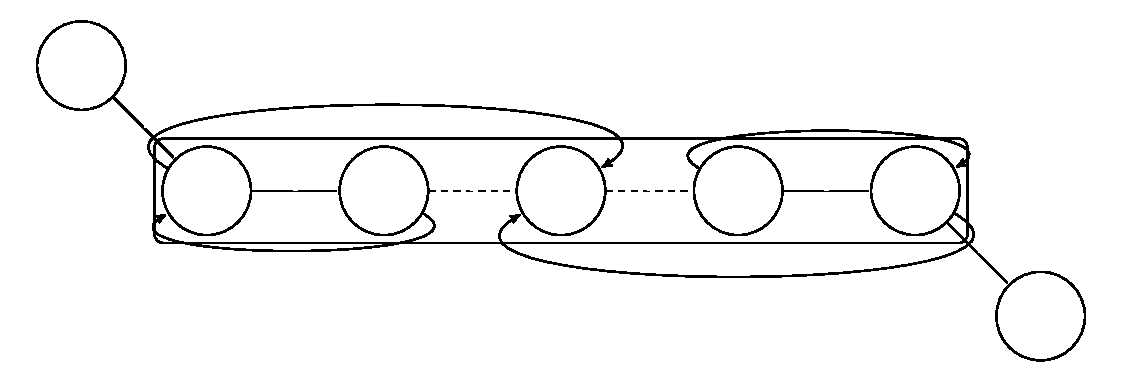
\includegraphics[scale=.7]{Imagenes/N7.pdf}
\caption{Movimientos de la vecindad N7}
\end{figure}
\end{itemize}

Las vecindades antes presentadas se han centrado en operaciones que pertenecen a la ruta crítica, esto les confiere las siguientes ventajas: la vecindad resultante es 
suficientemente pequeña como para ser explorada en su totalidad, para reducir el makespan de una planificación necesariamente deben hacerse cambios en la ruta crítica 
y en algunas de ellas puede garantizarse que cualquier vecino representa una solución factible~\cite{balas1969machine}.

%%TODO: Este párrafo quizás sobra o hay que buscar otro sitio donde colocarlo
%La literatura reciente se ha centrado en hacer los algoritmos existentes más eficientes dejando un poco de lado la parte de la representación o de la función de fitness. 
%%
%Existen otras ideas que no se han explorado a fondo pero parecen prometedoras como proponer extensiones a alguna de las vecindades que puedan considerar operaciones
%que no están en la ruta crítica, cambiar la representación o proponer una función de fitness que no solo tome en cuenta el makespan de modo que tengamos más formas de 
%diferenciar entre soluciones. 
%%
%Esta tesis pretende rellenar este vacío, y realizar estudios en torno a esas tres características.
%
%En la siguiente sección se presentan algunas otras medidas de calidad para planificaciones del JSP.

\subsection*{Criterios de optimalidad}
Como ya se ha mencionado el criterio de optimalidad más usado es el makespan, no obstante existen muchos otros criterios de optimalidad que pueden usarse para 
asignar un valor de fitness a una planificación. 

Si denotamos por $C_i$ al tiempo de finalización de la máquina $i$ y por $f_i(C_i)$ a un costo asociado, podemos distinguir dos tipos de funciones de 
costo en la literatura~\cite{Brucker2001}:
\[f_{\max}:=\max\{f_i(C_i)\}\]
y 
\[\sum f_i(C):=\sum_{1\leq i\leq n}f_i(C_i)\]

Los costos asociados a cada uno de los tiempos de finalización de los trabajos pueden tomar muchas formas, por ejemplo pueden introducirse pesos para cada 
trabajo o fijar tiempos de finalización esperado para cada trabajo y medir la desviación de ellos.
%
Dependiendo del problema en sí, puede ser que se le dé más o menos valor a distintos aspectos de la planificación como el tiempo que están detenidas las máquinas, 
o el tiempo que tarda un trabajo en particular. 
%
El makespan se ha usado ampliamente como criterio de optimalidad porque está muy relacionado con los costos económicos de la planificación~\cite{Rand1977}.


\section{Paisaje de búsqueda del JSP}

A partir de las definiciones anteriores sobre vecindades, función de aptitud y representaciones de las soluciones podemos construir el paisaje de búsqueda para el JSP.
%
Analizar el paisaje de búsqueda de un problema de optimización combinatoria puede ayudar a escoger o diseñar metaheurísticas aunque en la práctica resulta muy difícil
de hacer por el tamaño del espacio de soluciones. 
%
A la hora de analizar las características del paisaje de búsqueda ante diferentes parámetros de las instancias, a menudo presentan un un patrón 
\textit{fácil-difícil-fácil}~\cite{mammen1997new}, es decir, que para valores muy pequeños o grandes de ciertos parámetros el problema es fácil, y existen ciertos valores
intermedios, para los que el problema se hace difícil.

Para el caso particular del JSP se han realizado estudios con instancias pequeñas en los que se puede construir explícitamente todo el paisaje, i.e. se puede evaluar y 
construir la vecindad correspondiente a todas las soluciones. 
%
Con este paisaje construido pueden medirse cantidades de interés como la similitud entre óptimos locales o globales o el número de vecinos, entre otros, lo que da
pistas de la forma (como las mostradas en la figura \ref{fig:landtypes}) y dificultad del paisaje de búsqueda.
%
Se ha encontrado que el paisaje de búsqueda para instancias al azar sigue el patrón \textit{fácil-difícil-fácil} dependiendo de la razón entre el número de máquinas y 
número de trabajos de la misma~\cite{Streeter2006} ($\frac{N}{M}$) conforme esta cantidad  varía de 0 a infinito, siendo el caso más \textit{difícil} cuando $\frac{N}{M}\simeq 1$. 
%

Los experimentos computacionales sugieren que este patrón se da por cambios en la rugosidad del paisaje de búsqueda que se vuelve más y más pronunciada conforme $\frac{N}{M}$ crece.
%
Para valores pequeños se tiene un paisaje semejante a un gran valle suave, para valores grandes se tiene un pasaje con muchos óptimos locales pero todos ellos de buena calidad y 
para valores cercanos a 1 se tienen muchos óptimos locales de baja calidad.

También se ha encontrado que una de las características que hacen difícil a una instancia del JSP es la existencia de muchos óptimos locales de baja calidad que no son 
parecidos entre sí~\cite{mattfeld1999search}. 
%
Esto implica que sin importar el punto inicial de la metaheurística elegida rara vez estaremos muy lejos de uno de estos puntos. 
%
Otro factor que afecta el proceso de búsqueda local es que en general se ha encontrado que algunas soluciones están mucho mas conectadas que otras~\cite{bierwirth2004landscape}. 
%
Este último hecho puede ser tanto benéfico como perjudicial dependiendo si las soluciones altamente conectadas son de buena o mala calidad. 

Estas características explican en parte por qué los métodos basados en búsqueda local, como la búsqueda tabú, combinados con métodos sofisticados de exploración 
han tenido tan buenos resultados~\cite{watson2003problem}. 
%
Puede ser que las soluciones que estén más conectadas a otras sean de baja calidad y sea necesario evitar ser <<atraídos>> hacia ellas para llegar a soluciones de mejor calidad. 
%
También se ha observado que el paisaje de búsqueda para el JSP presenta grandes <<planicies>> i. e. zonas en las que todas las soluciones vecinas tienen el mismo makespan, 
en la práctica estas zonas actúan como un solo óptimo local que está altamente conectado.

En este sentido, podemos pensar que para que una metaheurística basada en búsqueda local tenga mayor probabilidad de encontrar buenas soluciones 
debemos plantear el paisaje de búsqueda de modo que no nos atasquemos en óptimos locales de muy mala calidad, ya sea porque conforman una planicie
amplia de la que es difícil salir o bien porque el paisaje de búsqueda es tan rugoso que hay óptimos locales por doquier y es fácil atascarse en uno de 
mala calidad. 

Ya que la dificultad de cada instancia puede variar, es importante contar con conjuntos de instancias que permitan evaluar el desempeño de los métodos de solución. 
%TODO: relacionarlo con los benchmarks

% strogatz small world networks
% figuras de grafos con buenas y malas características
